% Relatorio do ensaio de 24 h dos nos de qualidade do ar (telemetria-cria)
% Gerar:  cd python-dados && uv run python ../teste-24h/relatorio/gerar_graficos.py
%         cd ../teste-24h/relatorio && pdflatex relatorio.tex && pdflatex relatorio.tex
\documentclass[11pt,a4paper]{article}
\usepackage[T1]{fontenc}
\usepackage[utf8]{inputenc}
\usepackage[brazilian]{babel}
\usepackage[a4paper,top=22mm,bottom=22mm,left=22mm,right=22mm]{geometry}
\usepackage[scaled=0.92]{helvet}
\renewcommand{\familydefault}{\sfdefault}
\usepackage{textcomp}
\usepackage{courier}
\usepackage{microtype}
\usepackage[table]{xcolor}
\usepackage{graphicx}
\usepackage{booktabs}
\usepackage{array}
\usepackage{longtable}
\usepackage{tabularx}
\usepackage{enumitem}
\usepackage{float}
\usepackage{needspace}
\usepackage[font=small,labelfont=bf]{caption}
\usepackage[most]{tcolorbox}
\usepackage{fancyhdr}
\usepackage[hidelinks]{hyperref}

\definecolor{azul}{HTML}{1B64BE}
\definecolor{uso}{HTML}{EFEFEF}
\definecolor{cinza}{HTML}{4A4A4A}
\newcommand{\cod}{CO\textsubscript{2}}
\newcommand{\grau}{\,\textdegree C}
\newcommand{\no}[1]{\texttt{#1}}
\setlist{itemsep=2pt,topsep=4pt}
\setlength{\parskip}{6pt}
\setlength{\parindent}{0pt}
\renewcommand{\arraystretch}{1.15}
\pagestyle{fancy}
\fancyhf{}
\fancyhead[L]{\small\color{cinza}Ensaio de 24 h --- qualidade do ar em sala de aula}
\fancyhead[R]{\small\color{cinza}telemetria-cria}
\fancyfoot[C]{\small\color{cinza}\thepage}
\renewcommand{\headrulewidth}{0.3pt}
\newtcolorbox{destaque}[1][]{colback=azul!6,colframe=azul,boxrule=0.6pt,arc=2pt,left=8pt,right=8pt,top=6pt,bottom=6pt,#1}

\newcommand{\CoUsoMin}{400}
\newcommand{\CoUsoMed}{1.893}
\newcommand{\CoUsoMax}{4.327}
\newcommand{\MqUsoMin}{0,15}
\newcommand{\MqUsoMed}{0,42}
\newcommand{\MqUsoMax}{0,65}
\newcommand{\TeUsoMin}{27,7}
\newcommand{\TeUsoMed}{29,0}
\newcommand{\TeUsoMax}{29,9}
\newcommand{\UmUsoMin}{47}
\newcommand{\UmUsoMed}{55}
\newcommand{\UmUsoMax}{71}
\newcommand{\CoNoiteMin}{400}
\newcommand{\CoNoiteMed}{424}
\newcommand{\CoNoiteMax}{512}
\newcommand{\MqNoiteMin}{0,58}
\newcommand{\MqNoiteMed}{0,62}
\newcommand{\MqNoiteMax}{0,66}
\newcommand{\TeNoiteMin}{27,8}
\newcommand{\TeNoiteMed}{28,4}
\newcommand{\TeNoiteMax}{28,9}
\newcommand{\UmNoiteMin}{63}
\newcommand{\UmNoiteMed}{71}
\newcommand{\UmNoiteMax}{76}
\newcommand{\CoTudoMin}{400}
\newcommand{\CoTudoMed}{977}
\newcommand{\CoTudoMax}{4.327}
\newcommand{\MqTudoMin}{0,15}
\newcommand{\MqTudoMed}{0,54}
\newcommand{\MqTudoMax}{0,67}
\newcommand{\TeTudoMin}{26,5}
\newcommand{\TeTudoMed}{28,6}
\newcommand{\TeTudoMax}{29,9}
\newcommand{\UmTudoMin}{45}
\newcommand{\UmTudoMed}{63}
\newcommand{\UmTudoMax}{76}
\newcommand{\MinAcimaMil}{432}
\newcommand{\MinUsoAcimaMil}{432}
\newcommand{\HorasUsoAcimaMil}{7,2}
\newcommand{\PctUsoAcimaMil}{82}
\newcommand{\MinAcimaMilQuinhentos}{318}
\newcommand{\MinUsoAcimaMilQuinhentos}{318}
\newcommand{\HorasUsoAcimaMilQuinhentos}{5,3}
\newcommand{\PctUsoAcimaMilQuinhentos}{61}
\newcommand{\MinAcimaDoisMil}{242}
\newcommand{\MinUsoAcimaDoisMil}{242}
\newcommand{\HorasUsoAcimaDoisMil}{4,0}
\newcommand{\PctUsoAcimaDoisMil}{46}
\newcommand{\MinAcimaTresMil}{72}
\newcommand{\MinUsoAcimaTresMil}{72}
\newcommand{\HorasUsoAcimaTresMil}{1,2}
\newcommand{\PctUsoAcimaTresMil}{14}
\newcommand{\MinUso}{525}
\newcommand{\HorasUso}{8,75}
\newcommand{\PicoCo}{4.327}
\newcommand{\PicoCoHora}{13:38}
\newcommand{\RUso}{$-$0,68}
\newcommand{\RTudo}{$-$0,86}
\newcommand{\UmidAcimaSessentaCinco}{46}
\newcommand{\UmidUsoAcimaSessentaCinco}{2}
\newcommand{\TempAteVinteSeis}{0}
\newcommand{\PerdasNoSeisManha}{60}
\newcommand{\MqMenorMediaHora}{0,26}
\newcommand{\MqPctMenorMediaHora}{42}
\newcommand{\VazaoQuinze}{5}
\newcommand{\VazaoDezenove}{6}


\begin{document}

\thispagestyle{empty}
\vspace*{6mm}
{\color{azul}\rule{\linewidth}{2pt}}

\vspace{5mm}
{\Huge\bfseries Qualidade do ar em sala de aula\par}
\vspace{3mm}
{\Large Relatório do ensaio de 24 horas dos sensores de monitoramento\par}
\vspace{5mm}
{\large Projeto telemetria-cria --- Espaço Cria\par}
\vspace{2mm}
{\color{cinza}Período medido: das 17:47 de 25/11/2026 às 17:47 de 26/11/2026 (hora local)\\
Sensores: MQ-2, MH-Z19C, DHT22 e câmera ESP32-CAM\\
Emitido em 27/11/2026\par}
\vspace{5mm}
{\color{azul}\rule{\linewidth}{0.6pt}}

\vspace{5mm}
\begin{destaque}
\textbf{Resumo}

\begin{itemize}[leftmargin=*]
\item \textbf{Com a sala em uso, o \cod{} ficou acima de 1.000\,ppm em \PctUsoAcimaMil\,\% do tempo.} O \cod{} é o gás que as pessoas eliminam ao respirar; ao ar livre há cerca de 430\,ppm (partes por milhão), e 1.000\,ppm é o alvo usual para uma sala bem ventilada. Foram \HorasUsoAcimaMil\,horas acima de 1.000\,ppm e \HorasUsoAcimaDoisMil\,horas acima de 2.000\,ppm, com patamares de 3.500\,ppm no fim da manhã e no começo da tarde.
\item \textbf{A sala não renova o ar na proporção do número de pessoas.} Os níveis medidos são de ar abafado e de perda de atenção, não de intoxicação.
\item \textbf{A temperatura ficou acima de 26\grau{} as 24 horas} (de \TeTudoMin{} a \TeTudoMax\grau), e a umidade passou de 65\,\% durante a noite, com a sala fechada.
\item \textbf{O que fazer:} abrir portas e janelas por alguns minutos a cada aula e nos intervalos, usar o painel como aviso quando o \cod{} passar de 1.000\,ppm e avaliar com a manutenção uma entrada de ar externo (Seção~\ref{sec:recomendacoes}).
\item \textbf{Os valores vêm de sensores de baixo custo sem calibração de referência.} A ordem de grandeza e a forma das curvas são confiáveis; o valor exato de cada leitura, não.
\item \textbf{O sistema de medição funcionou as 24 horas sem intervenção.} Perdeu 0,20\,\% das leituras (limite: 1\,\%), mostrou os dados no painel em menos de 0,3\,s em 95\,\% das vezes (limite: 2\,s) e o servidor respondeu a 99,93\,\% das verificações (mínimo: 95\,\%).
\end{itemize}
\end{destaque}

\vfill
{\small\color{cinza}Os dados brutos estão na pasta \texttt{teste-24h/} do repositório claudin-rob (uma amostra por minuto) e no banco de dados do servidor (uma leitura a cada 10\,s). As figuras e os números deste relatório são gerados pelo script \texttt{gerar\_graficos.py}, na pasta \texttt{teste-24h/relatorio/}.}
\newpage

\tableofcontents
\newpage

% =====================================================================
\section{O que foi o ensaio}

O ensaio teve dois objetivos. O primeiro foi observar o que os sensores de qualidade do ar mostram em uma sala usada por alunos durante um dia de atividades. O segundo foi verificar se o sistema de telemetria (sensores com Wi-Fi, um servidor que recebe e guarda as medidas e um painel na web) funciona 24 horas seguidas sem intervenção.

Cada sensor está ligado a uma placa com Wi-Fi, chamada aqui de \emph{nó}, que envia as medidas ao servidor. Os quatro nós ficaram na mesma sala, ligados o tempo todo. A sala ficou vazia e fechada durante a noite e foi usada com alunos no dia 26/11. Nenhum equipamento foi reiniciado, regravado ou movido durante as 24 horas.

\begin{table}[H]
\centering\small
\begin{tabularx}{\linewidth}{@{}llXl@{}}
\toprule
\textbf{Nó} & \textbf{Sensor} & \textbf{O que mede} & \textbf{Intervalo} \\
\midrule
\no{no6} & MQ-2 & razão Rs/R0 (gases inflamáveis, vapores de álcool e fumaça) & 10\,s \\
\no{no7} & MH-Z19C & concentração de \cod{}, em ppm & 10\,s \\
\no{no8} & DHT22 (AM2302) & temperatura, em \textdegree C, e umidade relativa, em \% & 10\,s (cada grandeza) \\
\no{no10} & ESP32-CAM & foto da sala e contagem de fotos & 10\,min \\
\bottomrule
\end{tabularx}
\caption{Nós do ensaio. No servidor, eles estão registrados no projeto de nome \texttt{teste}.}
\label{tab:nos}
\end{table}

\textbf{Sobre o período de uso da sala.} Não houve registro de entrada e saída dos alunos. Neste relatório, ``sala em uso'' é o intervalo das 07:45 às 16:30 do dia 26/11 (\MinUso{} minutos), escolhido pelos próprios sensores. Às 07:45 a umidade e a temperatura começam a cair, sinal de ar-condicionado ligado, e dez minutos depois o \cod{} começa a subir. Às 16:28 o \cod{} fica de vez abaixo de 1.000\,ppm. O número de pessoas, o volume da sala e os horários em que portas, janelas e ar-condicionado foram abertos ou ligados não foram anotados.

% =====================================================================
\section{Grandezas medidas}

\subsection{Dióxido de carbono (\texorpdfstring{\cod}{CO2})}

O \cod{} é o gás que as pessoas eliminam ao respirar. Ao ar livre a concentração fica perto de 430\,ppm (partes por milhão), um pouco mais em área urbana. Em ambiente fechado ela sobe conforme o número de pessoas e desce conforme entra ar de fora. Por isso o \cod{} é usado como indicador de ventilação: quando ele está alto, o ar que as pessoas já respiraram não está sendo trocado, e junto com ele se acumulam odores, umidade e partículas que podem carregar vírus e bactérias.

O sensor MH-Z19C mede o \cod{} pela absorção de luz infravermelha. A faixa é de 400 a 5.000\,ppm, e a exatidão declarada pelo fabricante é de $\pm$(50\,ppm + 5\,\% da leitura). Ele não informa valores abaixo de 400\,ppm; por isso, uma leitura parada em 400\,ppm significa ``400 ou menos''.

\subsection{Razão Rs/R0 do MQ-2}

O MQ-2 é um sensor aquecido cuja resistência elétrica (Rs) cai quando há no ar gases inflamáveis ou vapores: gás de cozinha, hidrogênio, vapores de álcool, solventes e fumaça. Ele não distingue um gás do outro. O nó informa a razão entre a resistência medida e uma resistência de referência (R0). \textbf{Quanto menor a razão, maior a quantidade desses gases e vapores.}

Duas ressalvas valem para todo o relatório. O valor de R0 gravado no nó é provisório (18,2\,k$\Omega$, medido em bancada no dia 24/11), então a razão serve para comparar momentos, não para calcular concentrações. E a resposta do MQ-2 também muda com a temperatura e a umidade do ar.

\subsection{Temperatura e umidade relativa}

O DHT22 mede a temperatura do ar e a umidade relativa (quanto vapor de água o ar contém, em relação ao máximo que ele comporta naquela temperatura). A exatidão declarada é de $\pm$0,5\grau{} e de $\pm$2 a 5\,\% de umidade. As duas grandezas determinam o conforto térmico, e a umidade alta por muitas horas favorece mofo e ácaros.

\subsection{Grandezas do sistema de telemetria}

\begin{itemize}
\item \textbf{Perda de leituras:} cada leitura leva um número de sequência; os números que faltam no banco de dados são leituras perdidas.
\item \textbf{Latência:} tempo entre o nó fazer a leitura e o ponto aparecer desenhado no painel. O critério usa o \emph{percentil 95} (p95), que é o valor abaixo do qual ficaram 95\,\% das medidas; a \emph{mediana} é o valor abaixo do qual ficou a metade.
\item \textbf{Disponibilidade:} fração das verificações do servidor, feitas a cada 30\,s por um programa chamado aqui de \emph{verificador}, que tiveram resposta correta.
\end{itemize}

% =====================================================================
\section{Variação das grandezas ao longo das 24 horas}

A Figura~\ref{fig:grandezas} mostra as quatro grandezas nas 24 horas, e a Tabela~\ref{tab:comparacao} compara a noite com o período de uso. Os valores de cada hora estão no Apêndice~\ref{sec:horas}.

\begin{figure}[H]
\centering
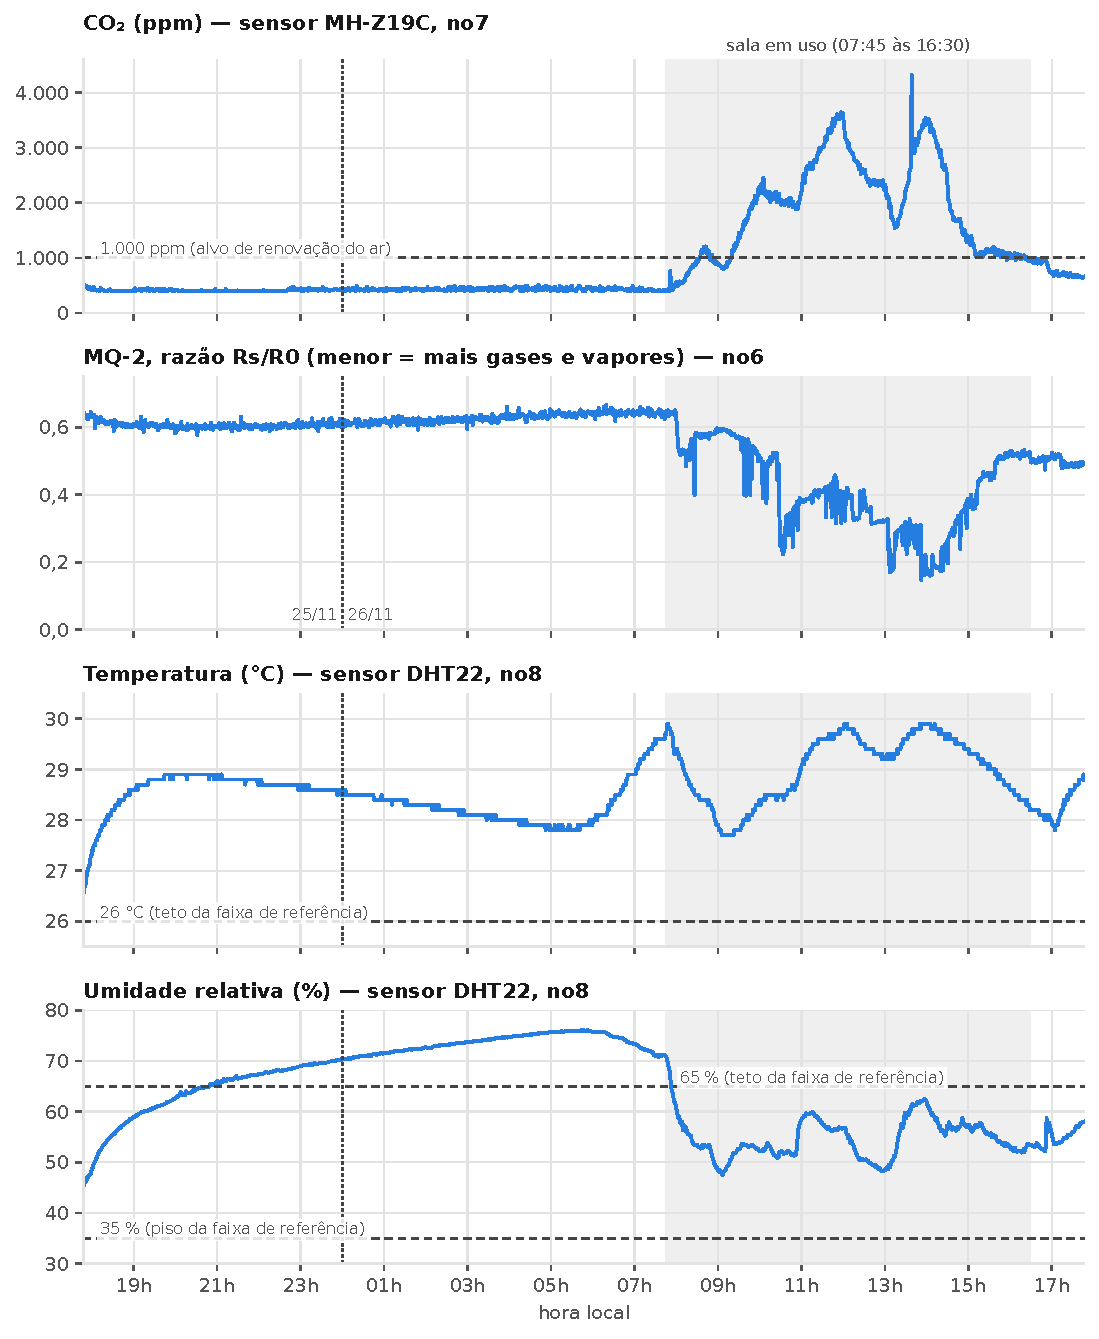
\includegraphics[width=\linewidth]{figuras/fig1_grandezas_24h.pdf}
\caption{As quatro grandezas ambientais, uma amostra por minuto. A faixa cinza marca a sala em uso e a linha vertical pontilhada, a meia-noite. As linhas tracejadas são os valores de referência da Seção~\ref{sec:referencias}.}
\label{fig:grandezas}
\end{figure}

\begin{table}[H]
\centering\small
\begin{tabular}{@{}lrrrrrr@{}}
\toprule
 & \multicolumn{3}{c}{\textbf{Noite, sala vazia (das 20h às 6h)}} & \multicolumn{3}{c}{\textbf{Sala em uso (07:45 às 16:30)}} \\
\cmidrule(lr){2-4}\cmidrule(l){5-7}
\textbf{Grandeza} & mínimo & média & máximo & mínimo & média & máximo \\
\midrule
\cod{} (ppm) & \CoNoiteMin & \CoNoiteMed & \CoNoiteMax & \CoUsoMin & \CoUsoMed & \CoUsoMax \\
MQ-2 (Rs/R0) & \MqNoiteMin & \MqNoiteMed & \MqNoiteMax & \MqUsoMin & \MqUsoMed & \MqUsoMax \\
Temperatura (\textdegree C) & \TeNoiteMin & \TeNoiteMed & \TeNoiteMax & \TeUsoMin & \TeUsoMed & \TeUsoMax \\
Umidade (\%) & \UmNoiteMin & \UmNoiteMed & \UmNoiteMax & \UmUsoMin & \UmUsoMed & \UmUsoMax \\
\bottomrule
\end{tabular}
\caption{Comparação entre a noite, com a sala vazia e fechada, e o período de uso.}
\label{tab:comparacao}
\end{table}

\subsection{Do fim da tarde ao amanhecer: sala vazia e fechada}

\begin{itemize}
\item \textbf{O \cod{} ficou no menor valor que o sensor informa ou pouco acima dele}, entre \CoNoiteMin{} e \CoNoiteMax\,ppm das 20h às 6h, com média de \CoNoiteMed\,ppm. Entre 20h e 22h o sensor ficou praticamente parado em 400\,ppm.
\item \textbf{O MQ-2 ficou estável}, entre \MqNoiteMin{} e \MqNoiteMax, subindo devagar ao longo da madrugada. Esse é o valor de base da sala sem pessoas.
\item \textbf{A temperatura subiu logo depois do início do ensaio}, de 26,5\grau{} às 17:47 para 28,9\grau{} duas horas depois, e caiu devagar até 27,8\grau{} às 5h. Entre 6h e 07:45 voltou a subir, até 29,9\grau, ainda com a sala vazia.
\item \textbf{A umidade subiu a noite inteira}, de 45\,\% no início do ensaio para 76\,\% de madrugada, e ficou acima de 65\,\% das 20:50 às 07:50.
\end{itemize}

A subida conjunta de temperatura e umidade no começo da noite é o comportamento esperado de uma sala climatizada depois que o ar-condicionado é desligado e a sala é fechada. Essa explicação é uma hipótese: o horário do ar-condicionado não foi anotado.

\subsection{O \texorpdfstring{\cod}{CO2} com a sala em uso}

\begin{figure}[H]
\centering
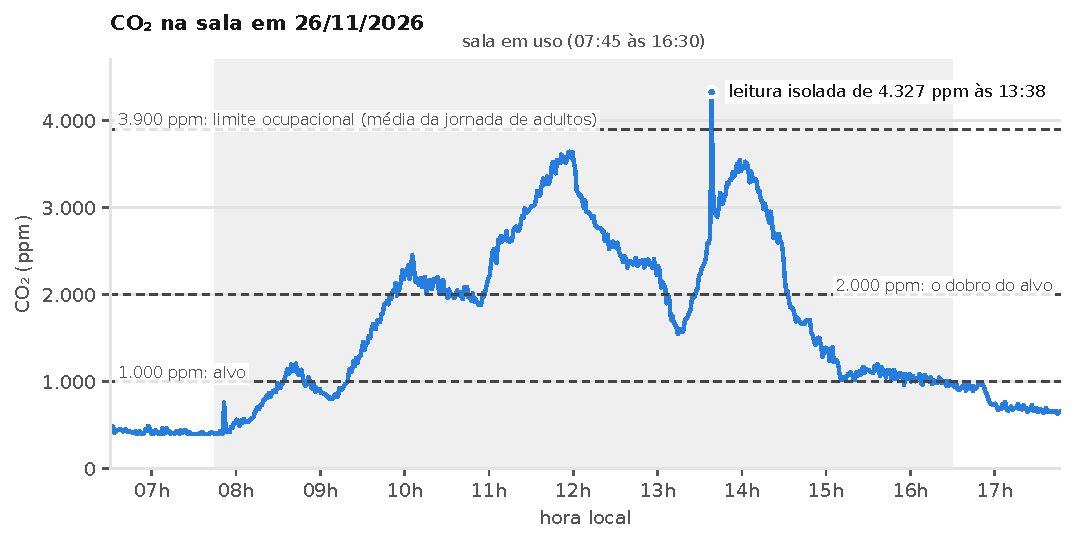
\includegraphics[width=\linewidth]{figuras/fig2_co2_dia.pdf}
\caption{\cod{} das 06:30 às 17:47 do dia 26/11. As linhas tracejadas em 1.000 e 2.000\,ppm são uma divisão prática adotada neste relatório (o alvo e o dobro dele); a de 3.900\,ppm é o limite ocupacional discutido na Seção~\ref{sec:referencias}.}
\label{fig:co2dia}
\end{figure}

A Figura~\ref{fig:co2dia} mostra o dia em detalhe:

\begin{itemize}
\item \textbf{07:45 a 09:10, chegada.} A umidade caiu de 71\,\% para 48\,\% e a temperatura, de 29,9 para 27,9\grau{}, o que indica ar-condicionado ligado. O \cod{} começou a subir às 07:55, passou de 1.000\,ppm pela primeira vez às 08:34, chegou a 1.200\,ppm e recuou para 800\,ppm às 09:08.
\item \textbf{09:10 a 10:05, primeira subida.} Em menos de uma hora o \cod{} foi de 800 para 2.450\,ppm, passando de 2.000\,ppm às 09:51.
\item \textbf{10:05 a 10:55, patamar.} O valor oscilou em torno de 2.000\,ppm, com leve queda até 1.900\,ppm.
\item \textbf{10:55 a 12:00, segunda subida.} O \cod{} foi de 1.900 para cerca de 3.600\,ppm (máximo de 3.643\,ppm às 11:57).
\item \textbf{12:00 a 13:15, queda parcial.} O valor desceu até cerca de 1.550\,ppm, o que é compatível com a saída de parte das pessoas ou com portas abertas no intervalo do almoço. Mesmo no ponto mais baixo, a sala continuou acima de 1.500\,ppm.
\item \textbf{13:15 a 14:30, segundo pico.} O \cod{} voltou a cerca de 3.500\,ppm às 14h. A leitura mais alta do ensaio, \PicoCo\,ppm às \PicoCoHora, ficou isolada, muito acima das leituras vizinhas, e provavelmente foi causada por alguém respirando perto do sensor; ela não representa o ar da sala.
\item \textbf{14:30 a 17:47, esvaziamento.} O \cod{} caiu para perto de 1.000\,ppm às 15:10, oscilou em torno desse valor por pouco mais de uma hora, ficou de vez abaixo dele às 16:28 e terminou o ensaio em cerca de 650\,ppm, ainda acima do valor da noite.
\end{itemize}

A Figura~\ref{fig:faixas} e a Tabela~\ref{tab:acima} resumem quanto tempo a sala passou em cada nível.

\begin{figure}[H]
\centering
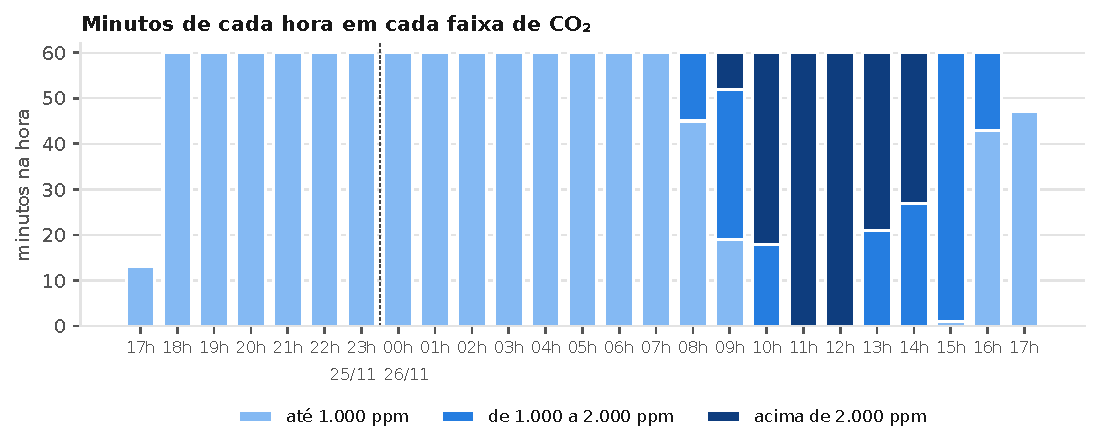
\includegraphics[width=\linewidth]{figuras/fig3_co2_faixas_hora.pdf}
\caption{Quantos minutos de cada hora o \cod{} passou em cada faixa. Das 11h às 12:59 a sala ficou o tempo todo acima de 2.000\,ppm. A primeira e a última barra são menores porque o ensaio começou e terminou às 17:47; por isso o rótulo 17h aparece duas vezes.}
\label{fig:faixas}
\end{figure}

\begin{table}[H]
\centering\small
\begin{tabular}{@{}lrrr@{}}
\toprule
\textbf{\cod{} acima de} & \textbf{Minutos} & \textbf{Horas} & \textbf{Parte do período de uso} \\
\midrule
1.000 ppm & \MinUsoAcimaMil & \HorasUsoAcimaMil & \PctUsoAcimaMil\,\% \\
1.500 ppm & \MinUsoAcimaMilQuinhentos & \HorasUsoAcimaMilQuinhentos & \PctUsoAcimaMilQuinhentos\,\% \\
2.000 ppm & \MinUsoAcimaDoisMil & \HorasUsoAcimaDoisMil & \PctUsoAcimaDoisMil\,\% \\
3.000 ppm & \MinUsoAcimaTresMil & \HorasUsoAcimaTresMil & \PctUsoAcimaTresMil\,\% \\
\bottomrule
\end{tabular}
\caption{Tempo acumulado acima de cada concentração, dentro dos \MinUso{} minutos de sala em uso. Fora desse período o \cod{} não passou de 1.000\,ppm.}
\label{tab:acima}
\end{table}

\subsection{O MQ-2 com a sala em uso}

\begin{figure}[H]
\centering
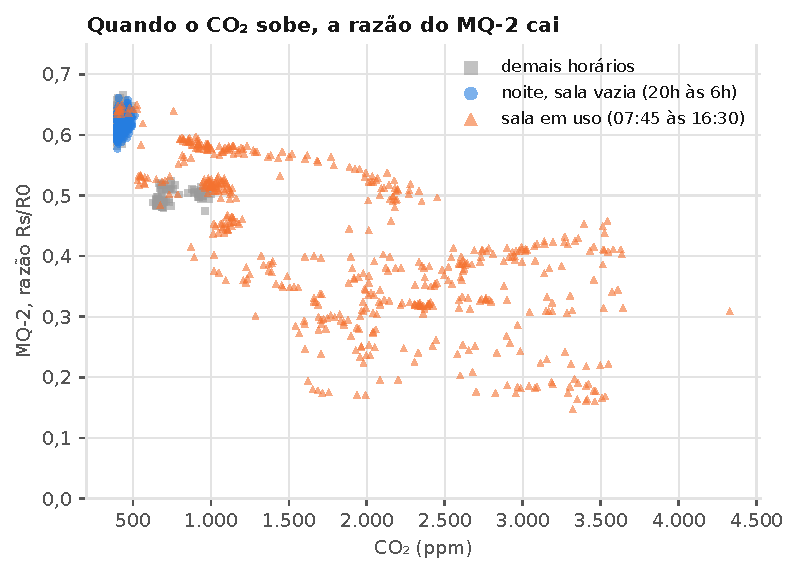
\includegraphics[width=0.74\linewidth]{figuras/fig4_co2_mq2.pdf}
\caption{Cada ponto é um minuto do ensaio. À noite os pontos ficam juntos no canto superior esquerdo; com a sala em uso, a razão do MQ-2 cai enquanto o \cod{} sobe. Os ``demais horários'' são o começo da noite de 25/11, o amanhecer e o fim da tarde de 26/11.}
\label{fig:mq2}
\end{figure}

A razão Rs/R0 caiu de cerca de \MqNoiteMed{} à noite para uma média de \MqUsoMed{} com a sala em uso. A hora de menor média (13h) ficou em \MqMenorMediaHora, cerca de \MqPctMenorMediaHora\,\% do valor noturno, e o menor valor instantâneo foi \MqUsoMin, às 13:52. A correlação com o \cod{} (Figura~\ref{fig:mq2}) é de \RTudo{} nas 24 horas e de \RUso{} dentro do período de uso; $-$1 seria uma relação inversa perfeita.

O MQ-2 não mede \cod{}. A queda da razão indica que, junto com as pessoas, aumentou a quantidade de compostos a que ele responde, como vapores de álcool (álcool em gel, perfumes, produtos de limpeza) e outros compostos orgânicos. As quedas bruscas e curtas, visíveis na Figura~\ref{fig:grandezas}, são típicas de fontes próximas e passageiras. O ensaio não permite dizer qual composto foi nem em que concentração.

\subsection{Temperatura e umidade com a sala em uso}

\begin{itemize}
\item \textbf{A temperatura ficou entre \TeUsoMin{} e \TeUsoMax\grau}, com média de \TeUsoMed\grau. Ela caiu cerca de 2\grau{} entre 07:45 e 09:05 e voltou a subir a partir das 09:30, acompanhando a ocupação da sala, até 29,9\grau{} por volta das 12h e das 14h.
\item \textbf{A umidade ficou entre \UmUsoMin{} e \UmUsoMax\,\%}, com média de \UmUsoMed\,\%. Ela só esteve acima de 65\,\% nos primeiros minutos, antes de o ar-condicionado fazer efeito; das 07:55 em diante ficou dentro da faixa de referência.
\end{itemize}

% =====================================================================
\section{Valores de referência}
\label{sec:referencias}

\begin{table}[H]
\centering\small
\begin{tabularx}{\linewidth}{@{}lXl@{}}
\toprule
\textbf{Grandeza} & \textbf{Referência} & \textbf{Fonte} \\
\midrule
\cod{} & até 700\,ppm acima da concentração do ar externo (cerca de 1.100 a 1.150\,ppm), como indicador de renovação do ar & ABNT NBR 17037:2023 \\
Temperatura & 21 a 26\grau & ABNT NBR 17037:2023 \\
Umidade relativa & 35 a 65\,\% & ABNT NBR 17037:2023 \\
\cod{} & 3.900\,ppm como média da jornada de trabalho de adultos (limite de tolerância, até 48 horas semanais) & NR-15, Anexo 11 \\
\bottomrule
\end{tabularx}
\caption{Valores de referência usados na análise.}
\label{tab:referencias}
\end{table}

\textbf{Sobre a norma brasileira.} A NBR 17037:2023 trata da qualidade do ar interior em ambientes não residenciais climatizados artificialmente. Ela substituiu a Resolução RE n.º 9/2003 da ANVISA, revogada em 2024 pela RDC n.º 886, que usava 1.000\,ppm fixos de \cod{}, 23 a 26\grau{} e 40 a 65\,\% de umidade no verão e pedia 27\,m\textsuperscript{3} de ar externo por hora para cada pessoa. A Lei n.º 13.589/2018 obriga os edifícios de uso público e coletivo com climatização a manter um Plano de Manutenção, Operação e Controle (PMOC) e a seguir esses parâmetros. Os valores da NBR 17037 foram tirados de um comunicado da ABRAVA sobre a mudança, e não do texto da norma, que é de acesso pago; convém conferi-los na norma antes de usá-los formalmente.

\textbf{Alvo usado neste relatório.} O relatório mantém 1.000\,ppm como alvo prático de \cod{}: é um valor redondo, próximo ao da norma atual e igual ao da resolução anterior. As faixas ``até 1.000'', ``de 1.000 a 2.000'' e ``acima de 2.000\,ppm'' são uma divisão adotada aqui para descrever os dados; não vêm de norma.

\textbf{Sobre o limite ocupacional.} O limite da NR-15 foi feito para caracterizar insalubridade no trabalho de adultos. Ele não é critério de conforto nem foi estabelecido para crianças e adolescentes; aparece aqui só para mostrar a distância entre os valores medidos e uma situação de risco direto.

\textbf{O que dizem os estudos.} Experimentos com adultos em ambientes que simulavam escritórios observaram queda no desempenho em tarefas de decisão com \cod{} em torno de 1.000\,ppm, e queda maior perto de 2.500\,ppm, em comparação com 550 a 600\,ppm (Satish e colaboradores, 2012; Allen e colaboradores, 2016). Outros experimentos não encontraram efeito do \cod{} puro até 3.000\,ppm, mas encontraram dor de cabeça, sonolência e pior desempenho quando a mesma concentração vinha de ventilação reduzida, isto é, acompanhada dos demais compostos que as pessoas exalam (Zhang e colaboradores, 2017). Uma revisão sobre escolas associa ventilação insuficiente a pior desempenho dos alunos e a mais faltas por doença (Fisk, 2017). Esses estudos justificam tratar 1.000\,ppm como alvo em sala de aula, mas não permitem prever o efeito sobre uma turma específica.

% =====================================================================
\section{Conclusões sobre a saúde do ambiente}
\label{sec:conclusoes}

\begin{destaque}
\textbf{1. A ventilação da sala é insuficiente para a ocupação que ela teve.} O \cod{} ficou acima do alvo de 1.000\,ppm em \PctUsoAcimaMil\,\% do período de uso e acima do dobro disso em \PctUsoAcimaDoisMil\,\%. Com ocupação constante, uma sala bem ventilada se estabiliza perto de 1.000\,ppm; esta chegou a 3.500\,ppm duas vezes no mesmo dia.
\end{destaque}

\textbf{2. A entrada de ar externo parece ser uma fração pequena do recomendado.} Um adulto sentado produz de 15 a 19 litros de \cod{} por hora. Para a sala se manter em 3.500\,ppm, a entrada de ar externo teria de ser de apenas \VazaoQuinze{} a \VazaoDezenove\,m\textsuperscript{3} por hora para cada pessoa, cerca de um quinto dos 27\,m\textsuperscript{3} que a resolução anterior pedia. É uma estimativa de ordem de grandeza: supõe adultos, ocupação constante e sala em equilíbrio, e crianças produzem menos \cod{}.

\textbf{3. Os níveis medidos são de ar abafado e de perda de atenção, não de intoxicação.} A média do período de uso foi de \CoUsoMed\,ppm, cerca de metade do limite ocupacional de 3.900\,ppm, e os patamares mais altos ficaram abaixo dele. Nessas condições, o que os estudos relatam é sensação de ar abafado, sonolência, dor de cabeça e dificuldade de concentração. A evidência é mais consistente para o conjunto do ar mal renovado do que para o \cod{} isolado, e nem todas as pessoas sentem esses efeitos.

\textbf{4. O \cod{} alto indica que o ar exalado está sendo respirado de novo.} Quanto maior o \cod{}, maior a fração do ar da sala que já passou pelos pulmões de alguém. Isso aumenta o risco de transmissão de doenças respiratórias pelo ar quando há alguém infectado na sala. O \cod{} indica esse risco, mas não mede vírus nem leva em conta máscaras ou filtragem.

\textbf{5. A sala esteve quente o tempo todo.} A temperatura não ficou abaixo de 26\grau{} em nenhum momento das 24 horas e chegou a 29,9\grau{} tanto com a sala cheia quanto no começo da manhã, ainda vazia. Com a sala em uso, isso aconteceu mesmo com sinais de ar-condicionado ligado. O calor soma-se ao ar mal renovado na sensação de abafamento.

\textbf{6. À noite, a sala fechada ficou úmida.} A umidade passou de 65\,\% em \UmidAcimaSessentaCinco\,\% das 24 horas, quase sempre com a sala vazia, e chegou a 76\,\%. Umidade acima de 60 a 65\,\% por muitas horas, noite após noite, favorece mofo e ácaros, que agravam rinite e asma. Um único dia não basta para dizer que isso acontece sempre.

\textbf{7. O MQ-2 confirma a mudança do ar com a ocupação, mas não serve para avaliar risco.} A razão caiu para cerca de \MqPctMenorMediaHora\,\% do valor noturno na hora de maior ocupação, com mínimos momentâneos de um quarto. O padrão, de queda gradual acompanhando a ocupação com picos curtos, é o de compostos trazidos pelas pessoas e pelos produtos que elas usam, e não o de um vazamento contínuo. Sem calibração, porém, o MQ-2 não permite afirmar nem descartar perigo: ele não substitui detector de gás nem de fumaça.

\textbf{8. A combinação observada é a de sala fechada com ar-condicionado sem entrada de ar externo.} Aparelhos do tipo \emph{split} resfriam e secam o ar, mas apenas o recirculam. Os dados são coerentes com isso: a umidade caiu assim que a sala começou a ser usada, enquanto o \cod{} subiu. Essa interpretação precisa ser confirmada no local.

% =====================================================================
\needspace{12\baselineskip}
\section{Recomendações}
\label{sec:recomendacoes}

\enlargethispage{2\baselineskip}
\begin{itemize}
\item \textbf{Abrir portas e janelas por alguns minutos a cada aula} e deixar a sala aberta nos intervalos. No horário do almoço o \cod{} caiu de 3.600 para 1.550\,ppm, o que mostra que a sala responde quando o ar circula ou a ocupação diminui. É uma medida paliativa: ela traz calor e umidade que o ar-condicionado precisa retirar.
\item \textbf{Avaliar com a manutenção uma entrada de ar externo} (renovação mecânica ou exaustor), dimensionada para a ocupação máxima da sala. Esta é a solução de fato. Vale levar este resultado ao responsável pelo PMOC do prédio.
\item \textbf{Reduzir a ocupação ou dividir as turmas} nas atividades mais longas, enquanto não houver entrada de ar externo.
\item \textbf{Usar o painel como aviso de ventilação.} Um sinal visual quando o \cod{} passar de 1.000\,ppm, e outro em 2.000\,ppm, dá à turma um critério objetivo para abrir a sala. Antes disso, calibrar o zero do MH-Z19C ao ar livre e, se possível, compará-lo com um medidor de referência.
\item \textbf{Acompanhar a umidade noturna sem contar com a ventilação natural para secar a sala.} Em Recife o ar de fora costuma ser mais úmido que o de uma sala climatizada. Observar sinais de mofo (cantos, forro, atrás de armários, filtros do ar-condicionado), manter a limpeza de filtros e bandeja prevista no PMOC e repetir a medição por vários dias, de preferência com um sensor do lado de fora.
\item \textbf{Registrar a ocupação nos próximos ensaios}: número de pessoas, horários de entrada e saída, estado de portas, janelas e ar-condicionado. Com esses dados e o volume da sala é possível calcular a taxa de renovação de ar, em vez de estimá-la.
\end{itemize}

% =====================================================================
\section{Desempenho do sistema de telemetria}
\label{sec:telemetria}

O projeto telemetria-cria tem seis critérios de aceitação definidos no seu plano de trabalho. Três deles podem ser medidos automaticamente e são os avaliados aqui (Tabela~\ref{tab:criterios}); os outros três (exatidão do pH, exatidão da condutividade e reúso) dependem de medidas manuais e não fizeram parte deste ensaio.

\begin{table}[H]
\centering\small
\begin{tabularx}{\linewidth}{@{}lllX@{}}
\toprule
\textbf{Critério} & \textbf{Exigido} & \textbf{Medido} & \textbf{Situação} \\
\midrule
1. Perda de leituras & menos de 1\,\% & 0,20\,\% (70 de 34.843) & atende nos números \\
2. Latência & p95 abaixo de 2\,s & p95 de 207\,ms; mediana de 59\,ms & atende \\
5. Disponibilidade & pelo menos 95\,\% & 99,93\,\% (2.878 de 2.880 verificações) & atende \\
\bottomrule
\end{tabularx}
\caption{Critérios automáticos do teste de aceitação nas 24 horas. No critério 1, o relatório automático pede conferência manual por causa de dois avisos sobre a câmera, que envia dados só a cada 10 minutos; os avisos são esperados para esse nó.}
\label{tab:criterios}
\end{table}

\begin{table}[H]
\centering\small
\begin{tabular}{@{}lrrrr@{}}
\toprule
\textbf{Nó} & \textbf{Esperadas} & \textbf{Recebidas} & \textbf{Perdidas} & \textbf{Perda} \\
\midrule
\no{no6} (MQ-2) & 8.637 & 8.573 & 64 & 0,74\,\% \\
\no{no7} (MH-Z19C) & 8.640 & 8.638 & 2 & 0,02\,\% \\
\no{no8} (DHT22) & 17.278 & 17.274 & 4 & 0,02\,\% \\
\no{no10} (câmera) & 288 & 288 & 0 & 0,00\,\% \\
\midrule
Total & 34.843 & 34.773 & 70 & 0,20\,\% \\
\bottomrule
\end{tabular}
\caption{Perda de leituras por nó. Nenhum nó reiniciou durante o ensaio. A câmera envia duas leituras a cada foto (contagem de fotos e fotos pendentes): 144 fotos, 288 leituras.}
\label{tab:perda}
\end{table}

\begin{figure}[H]
\centering
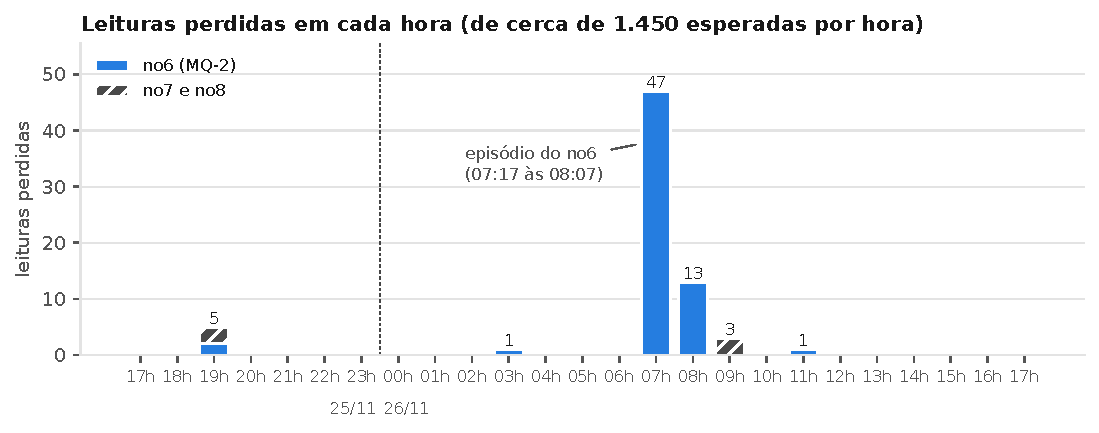
\includegraphics[width=\linewidth]{figuras/fig5_perdas_hora.pdf}
\caption{Leituras perdidas em cada hora. O rótulo 17h aparece duas vezes porque o ensaio começou e terminou às 17:47.}
\label{fig:perdas}
\end{figure}

\textbf{O que os números mostram}

\begin{itemize}
\item \textbf{Quase toda a perda veio de um episódio só} (Figura~\ref{fig:perdas}). Entre 07:17 e 08:07 do dia 26, o \no{no6} perdeu \PerdasNoSeisManha{} leituras e ficou sem conexão 11 vezes, por 1 a 2 minutos cada vez. Ele não reiniciou e os outros três nós não foram afetados. O episódio começou cerca de meia hora antes dos primeiros sinais de ocupação da sala. A causa não foi confirmada; as hipóteses são interferência no sinal Wi-Fi desse nó ou mau contato na alimentação.
\item \textbf{Houve duas oscilações curtas do Wi-Fi}, às 19:12 do dia 25 e às 09:51 do dia 26, em que mais de um nó perdeu 1 ou 2 leituras no mesmo minuto.
\item \textbf{A latência ficou cerca de dez vezes abaixo do limite.} O painel mediu a latência de 34.688 das 34.735 leituras que chegaram ao vivo (99,9\,\%). O percentil 99 foi de 1,18\,s e a maior latência, de 7,59\,s; 99,8\,\% das medidas ficaram abaixo de 2\,s.
\item \textbf{O servidor não caiu.} As duas verificações contadas como falhas (20:05 e 11:00) tiveram resposta correta imediatamente antes e depois; o relógio do verificador escorregou cerca de 1\,s e aquele intervalo de 30\,s ficou sem consulta.
\item \textbf{A câmera enviou todas as fotos.} Foram 144 fotos nas 24 horas, uma a cada 10 minutos, todas gravadas no cartão de memória e recebidas pelo servidor.
\end{itemize}

\textbf{Limite desta medição.} O verificador rodou no mesmo computador do servidor, então mede se o serviço está de pé, mas não detecta queda da rede entre o servidor e outros computadores. As ocorrências estão listadas no Apêndice~\ref{sec:ocorrencias}.

% =====================================================================
\section{Limitações}

\begin{itemize}
\item \textbf{Um único dia e um único ponto de medição.} Os sensores ficaram juntos, em um só lugar da sala. A concentração pode variar entre o fundo e a frente da sala e conforme a altura.
\item \textbf{O MH-Z19C não foi comparado com um instrumento de referência.} O sensor se recalibra sozinho, tomando o menor valor de cada 24 horas como 400\,ppm. Como ele passou horas parado em 400\,ppm, é provável que o zero esteja deslocado para baixo, o que faria as leituras do dia marcarem menos do que o real. Já o erro proporcional (até cerca de $\pm$225\,ppm em 3.500\,ppm) pode ir para qualquer lado. E, como a recalibração força o mínimo a 400\,ppm, os valores noturnos não provam, por si, que a sala voltou ao nível do ar externo.
\item \textbf{O MQ-2 usa um R0 provisório} e responde a vários gases, à temperatura e à umidade. Ele serve como indicador de mudança, não como medida de concentração.
\item \textbf{O DHT22 também não foi calibrado.} Montado perto de uma placa eletrônica, que aquece, ele pode marcar alguns décimos de grau a mais do que o ar da sala.
\item \textbf{O ensaio não mediu tudo o que define a qualidade do ar.} Ficaram de fora poeira fina (material particulado), compostos orgânicos específicos e contaminação por fungos e bactérias. \cod{} baixo não garante ar limpo; \cod{} alto garante que a renovação é insuficiente.
\item \textbf{O período de uso foi inferido pelos sensores}, e não por registro de presença. As explicações que envolvem ar-condicionado, portas e número de pessoas são hipóteses coerentes com os dados, não fatos observados.
\item \textbf{As referências citadas valem para ambientes climatizados em geral e, no caso do limite ocupacional, para adultos.} Elas são usadas aqui como referência de boa prática, não como laudo.
\end{itemize}

Este relatório descreve um ensaio didático. Ele não substitui uma avaliação de qualidade do ar feita por profissional habilitado com instrumentos calibrados.

% =====================================================================
\section*{Referências}
\addcontentsline{toc}{section}{Referências}

{\small\raggedright
\begin{itemize}[leftmargin=*]
\item ABNT. \emph{NBR 17037:2023 --- Qualidade do ar interior em ambientes não residenciais climatizados artificialmente: padrões referenciais}.
\item ABRAVA. \emph{Comunicado de alterações na legislação brasileira sobre qualidade do ar interno}, 5 ago. 2024.
\item ANVISA. \emph{Resolução RE n.º 9, de 16 de janeiro de 2003} (revogada pela RDC n.º 886/2024).
\item BRASIL. \emph{Lei n.º 13.589, de 4 de janeiro de 2018} (Plano de Manutenção, Operação e Controle de sistemas de climatização).
\item BRASIL. Ministério do Trabalho e Emprego. \emph{NR-15, Anexo 11 --- Agentes químicos cuja insalubridade é caracterizada por limite de tolerância}.
\item ALLEN, J. G. et al. Associations of cognitive function scores with carbon dioxide, ventilation, and volatile organic compound exposures in office workers. \emph{Environmental Health Perspectives}, v. 124, n. 6, 2016.
\item FISK, W. J. The ventilation problem in schools: literature review. \emph{Indoor Air}, v. 27, n. 6, 2017.
\item PERSILY, A.; DE JONGE, L. Carbon dioxide generation rates for building occupants. \emph{Indoor Air}, v. 27, n. 5, 2017.
\item SATISH, U. et al. Is CO\textsubscript{2} an indoor pollutant? Direct effects of low-to-moderate CO\textsubscript{2} concentrations on human decision-making performance. \emph{Environmental Health Perspectives}, v. 120, n. 12, 2012.
\item ZHANG, X.; WARGOCKI, P.; LIAN, Z. et al. Effects of exposure to carbon dioxide and bioeffluents on perceived air quality, self-assessed acute health symptoms, and cognitive performance. \emph{Indoor Air}, v. 27, n. 1, 2017.
\item WINSEN. \emph{MH-Z19C NDIR CO\textsubscript{2} sensor: user's manual}.
\end{itemize}
}

% =====================================================================
\appendix
\section{Valores por hora}
\label{sec:horas}

{\small
\begin{longtable}{@{}lrrrrrrrr@{}}
\toprule
 & \multicolumn{2}{c}{\textbf{\cod{} (ppm)}} & \multicolumn{2}{c}{\textbf{MQ-2 (Rs/R0)}} & \multicolumn{2}{c}{\textbf{Temp. (\textdegree C)}} & \multicolumn{2}{c}{\textbf{Umidade (\%)}} \\
\cmidrule(lr){2-3}\cmidrule(lr){4-5}\cmidrule(lr){6-7}\cmidrule(l){8-9}
\textbf{Hora} & média & máx. & média & mín. & média & máx. & média & máx. \\
\midrule
\endhead
25/11 17h & 463 & 502 & 0,63 & 0,62 & 26,9 & 27,3 & 47 & 49 \\
25/11 18h & 408 & 472 & 0,61 & 0,59 & 28,1 & 28,6 & 55 & 59 \\
25/11 19h & 418 & 452 & 0,60 & 0,58 & 28,8 & 28,9 & 61 & 63 \\
25/11 20h & 402 & 438 & 0,60 & 0,58 & 28,9 & 28,9 & 64 & 66 \\
25/11 21h & 401 & 433 & 0,60 & 0,59 & 28,8 & 28,9 & 67 & 67 \\
25/11 22h & 411 & 477 & 0,60 & 0,59 & 28,7 & 28,8 & 68 & 69 \\
25/11 23h & 425 & 468 & 0,61 & 0,59 & 28,6 & 28,7 & 70 & 70 \\
26/11 00h & 424 & 486 & 0,61 & 0,60 & 28,5 & 28,6 & 71 & 72 \\
26/11 01h & 427 & 458 & 0,62 & 0,59 & 28,4 & 28,4 & 72 & 73 \\
26/11 02h & 432 & 493 & 0,62 & 0,59 & 28,2 & 28,3 & 73 & 74 \\
26/11 03h & 437 & 489 & 0,63 & 0,61 & 28,1 & 28,1 & 74 & 75 \\
26/11 04h & 443 & 512 & 0,63 & 0,61 & 27,9 & 28,0 & 75 & 76 \\
26/11 05h & 437 & 493 & 0,64 & 0,63 & 27,8 & 28,0 & 76 & 76 \\
26/11 06h & 432 & 491 & 0,64 & 0,62 & 28,4 & 28,9 & 75 & 76 \\
\rowcolor{uso}26/11 07h & 426 & 761 & 0,64 & 0,62 & 29,4 & 29,9 & 70 & 73 \\
\rowcolor{uso}26/11 08h & 861 & 1.207 & 0,56 & 0,40 & 28,6 & 29,4 & 54 & 61 \\
\rowcolor{uso}26/11 09h & 1.401 & 2.279 & 0,55 & 0,40 & 27,9 & 28,4 & 51 & 54 \\
\rowcolor{uso}26/11 10h & 2.079 & 2.451 & 0,40 & 0,22 & 28,6 & 29,0 & 53 & 58 \\
\rowcolor{uso}26/11 11h & 3.032 & 3.643 & 0,40 & 0,31 & 29,5 & 29,8 & 58 & 60 \\
\rowcolor{uso}26/11 12h & 2.631 & 3.512 & 0,35 & 0,31 & 29,5 & 29,9 & 51 & 57 \\
\rowcolor{uso}26/11 13h & 2.464 & 4.327 & 0,26 & 0,15 & 29,6 & 29,9 & 57 & 63 \\
\rowcolor{uso}26/11 14h & 2.357 & 3.528 & 0,26 & 0,16 & 29,7 & 29,9 & 58 & 62 \\
\rowcolor{uso}26/11 15h & 1.119 & 1.396 & 0,46 & 0,36 & 29,0 & 29,4 & 55 & 58 \\
\rowcolor{uso}26/11 16h & 957 & 1.089 & 0,51 & 0,47 & 28,3 & 28,6 & 53 & 59 \\
26/11 17h & 684 & 768 & 0,50 & 0,48 & 28,4 & 28,9 & 56 & 58 \\
\bottomrule
\caption{Estatísticas de cada hora do ensaio. As linhas em cinza são as horas que têm algum trecho do período de uso (07:45 às 16:30). A primeira e a última linha cobrem só parte da hora, porque o ensaio começou e terminou às 17:47.}\label{tab:horas}
\end{longtable}
}


\section{Ocorrências registradas durante o ensaio}
\label{sec:ocorrencias}

Um programa de monitoramento consultou o painel uma vez por minuto e anotou cada problema ao começar e ao terminar. O arquivo completo, com 62 linhas, é \texttt{teste-24h/erros.log}. A Tabela~\ref{tab:ocorrencias} resume o que ele registrou.

\begin{table}[H]
\centering\small
\begin{tabularx}{\linewidth}{@{}llX@{}}
\toprule
\textbf{Quando} & \textbf{Nó} & \textbf{Ocorrência} \\
\midrule
25/11 19:06 & \no{no6} & 1 leitura perdida \\
25/11 19:12 & \no{no6}, \no{no7}, \no{no8} & 4 leituras perdidas no mesmo minuto (1, 1 e 2) \\
25/11 19:14 & \no{no10} & página da câmera inacessível por 1 minuto; fotos não afetadas \\
25/11 20:05 & servidor & intervalo de 30\,s sem consulta do verificador (servidor respondendo) \\
26/11 03:51 & \no{no6} & 1 leitura perdida \\
26/11 07:17 a 08:07 & \no{no6} & 60 leituras perdidas; 11 quedas de conexão de 1 a 2 minutos; maior lacuna de 12 leituras às 07:35; duas vezes sem leitura nova por mais de 60\,s \\
26/11 09:51 & \no{no7}, \no{no8} & 3 leituras perdidas no mesmo minuto (1 e 2) \\
26/11 11:00 & servidor & intervalo de 30\,s sem consulta do verificador (servidor respondendo) \\
26/11 11:11 & \no{no6} & 1 leitura perdida \\
\bottomrule
\end{tabularx}
\caption{Resumo das ocorrências das 24 horas.}
\label{tab:ocorrencias}
\end{table}

\section{Como reproduzir}

{\raggedright
\textbf{Dados.} Na pasta \texttt{teste-24h/}: amostras por minuto no arquivo \texttt{amostras.jsonl} e ocorrências no arquivo \texttt{erros.log}. As consultas de disponibilidade ficam na pasta \texttt{validacao/dados/} do repositório telemetria-cria.

\textbf{Critérios de aceitação.} Na pasta \texttt{servidor/} da telemetria-cria; o resultado está no arquivo \texttt{relatorio-final-24h.md}:

{\footnotesize\ttfamily npm run relatorio -{}- -{}-inicio 2026-11-25T17:47 \textbackslash\\
\hspace*{2em}-{}-fim 2026-11-26T17:47 -{}-projetos teste\par}

\textbf{Figuras e números deste relatório.} A partir da pasta \texttt{python-dados/}:

{\footnotesize\ttfamily uv run python ../teste-24h/relatorio/gerar\_graficos.py\par}

Depois, na pasta \texttt{teste-24h/relatorio/}, rodar \texttt{pdflatex relatorio.tex} duas vezes.\par}

\end{document}
